\documentclass[tikz, border=2mm]{standalone}

%\usepackage[english]{babel}
\usepackage{tikz}
\usepackage{amsmath}
\usepackage{amsfonts}
\usepackage{amssymb}
%\usepackage{pgfplots}

\usetikzlibrary{shapes.geometric}
\usetikzlibrary{calc}
\usetikzlibrary{cd}
\usetikzlibrary{automata, positioning, arrows}

\tikzset{
    ->, % makes the edges directed
    >=stealth', % makes the arrow heads bold
    node distance=3cm, % specifies the minimum distance between two nodes. Change if necessary.
    every state/.style={thick, fill=gray!10}, % sets the properties for each 'state' node
    initial text=$ $, % sets the text that appears on the start arrow
}

%\pgfplotsset{compat=1.12}
\begin{document}
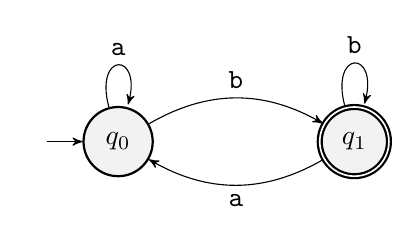
\begin{tikzpicture}
    \node[state, initial](q0){\(q_0\)};
    \node[state, accepting,right of=q0](q1){\(q_1\)};

    \draw (q0) edge[loop above] node{{\tt a}} (q0);
    \draw (q1) edge[loop above] node{{\tt b}} (q1);
    \draw (q0) edge[bend left, above] node{{\tt b}} (q1);
    \draw (q1) edge[bend left, below] node{{\tt a}} (q0);
\end{tikzpicture}
\end{document}